\documentclass[12pt]{article}
\usepackage{float}
\usepackage{graphicx}
\usepackage{geometry}
\usepackage{listings}
\usepackage{xcolor}
\geometry{margin=1in}
\usepackage{amsmath}
\usepackage{circuitikz}
\usepackage{url}
\title{Assignment 2}
\author{Arnav Yadnopavit\\EE24BTECH11007}
\date{\today}

\lstset{
  basicstyle=\ttfamily\small,
  keywordstyle=\color{blue},
  commentstyle=\color{gray},
  stringstyle=\color{red},
  showstringspaces=false,
  breaklines=true,
  frame=single,
  language=Verilog
}

\begin{document}

\maketitle

\section{Problem 1: Convolution of Two 8-element Vectors}
\subsection*{Objective}
Design a Verilog module to perform discrete convolution on two 8-element input vectors (4-bit each).

\subsection*{Code}
\textbf{1\_convolution.v}
\lstinputlisting{codes/1/1_convolution.v}


\textbf{1\_test.v}
\lstinputlisting{codes/1/1_test.v}
\begin{figure}[H]
    \centering
    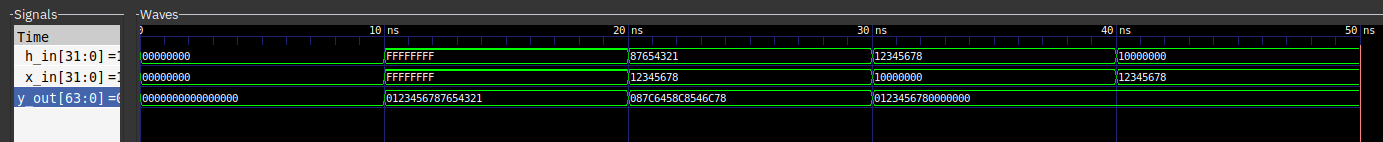
\includegraphics[width=\textwidth]{figs/1/test.png} 
    \caption{Timing Diagram}
\end{figure}
\subsection*{Explanation}
This module performs a discrete convolution using nested loops over two 8-element arrays. For each output index, it computes the sum of products of overlapping elements. Overflow is ignored by truncating the result to 4 bits.

\section{Problem 2: 8-bit Full Adder Using Loop}
\subsection*{Objective}
Design an 8-bit full adder using generate block (loop statement).

\subsection*{Code}
\textbf{2\_adder.v}
\lstinputlisting{codes/2/2_adder.v}

\textbf{2\_test.v}
\lstinputlisting{codes/2/2_test.v}
\begin{figure}[H]
    \centering
    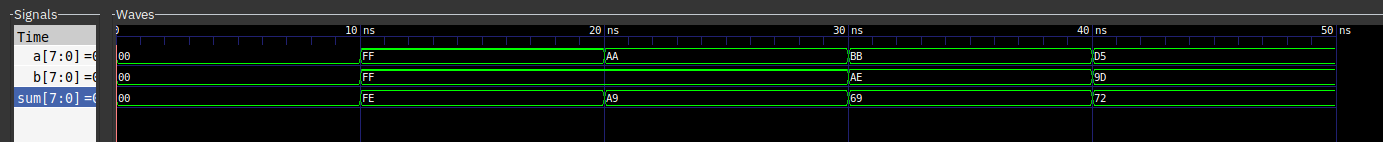
\includegraphics[width=\textwidth]{figs/2/test.png} 
    \caption{Timing Diagram}
\end{figure}
\subsection*{Explanation}
The adder uses a generate block to instantiate 8 full adders for each bit. Carry propagates through a wire array. No arithmetic operators are used.

\section{Problem 3: 4-bit Ripple Carry Adder using NAND Gates}
\subsection*{Objective}
Create a 4-bit ripple carry adder using only 2-input NAND gates with 1 ns delay.

\subsection*{Code}
\textbf{3\_nandcounter.v}
\lstinputlisting{codes/3/3_nandcounter.v}

\textbf{3\_test.v}
\lstinputlisting{codes/3/3_test.v}
\begin{figure}[H]
    \centering
    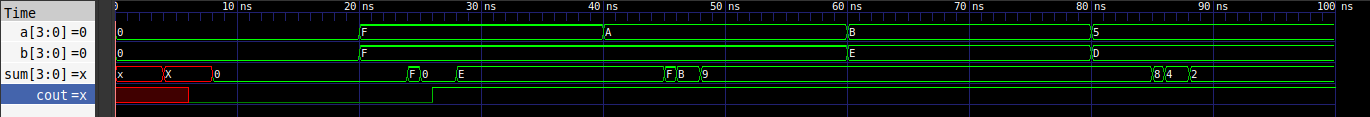
\includegraphics[width=\textwidth]{figs/3/test.png} 
    \caption{Timing Diagram}
\end{figure}
\subsection*{Explanation}
The 4-bit ripple carry adder is implemented entirely using 2-input NAND gates. XOR, AND, and OR gates are constructed from NANDs. Delay per gate is set to 1 ns, and the ripple-carry effect propagates through the bitadder stages. Each bit's carry is passed to the next stage, emulating the behavior of a ripple-carry adder structurally.
\section*{Propagation Delay Analysis}

\subsection*{Gate Delay Assumptions}
Each 2‑input NAND gate has a delay of 1\,ns. All logic gates are built from these NANDs:
\[
  \begin{aligned}
    \text{XOR (4 NANDs)} &\Rightarrow 4 \times 1\,\text{ns} = 4\,\text{ns},\\
    \text{AND (3 NANDs)} &\Rightarrow 3 \times 1\,\text{ns} = 3\,\text{ns},\\
    \text{OR  (3 NANDs)} &\Rightarrow 3 \times 1\,\text{ns} = 3\,\text{ns}.
  \end{aligned}
\]

\subsection*{Full Adder (\texttt{bitadder}) Delay}
Each 1‑bit full adder has two paths:
\[
  \begin{aligned}
    \text{Sum path:}  &\quad 2\;\text{XORs}
      = 4\,\text{ns} + 4\,\text{ns}
      = 8\,\text{ns},\\
    \text{Carry path:}&\quad 3\;\text{ANDs} + 2\;\text{ORs}
      = 3\times3\,\text{ns} + 2\times3\,\text{ns}
      = 9\,\text{ns} + 6\,\text{ns}
      = 15\,\text{ns}.
  \end{aligned}
\]

\subsection*{Worst‑Case Delay for 4‑bit Ripple Carry Adder}
The carry ripples through three full‑adder stages before the final sum bit:
\[
  \text{Total worst‑case delay}
    = 4 \times (\text{carry delay}) + (\text{sum delay})
    = 4 \times 15\,\text{ns} + 4 \times 8\,\text{ns}
    = \boxed{82\,\text{ns}}.
\]
\section*{Module Gatelevel Diagrams}
\subsection{XOR}
\begin{figure}[H]
\centering
\resizebox{1\textwidth}{!}{%
\begin{circuitikz}
\tikzstyle{every node}=[font=\large]

\draw (9.75,13.25) to[short] (10,13.25);
\draw (9.75,12.75) to[short] (10,12.75);
\draw (10,13.25) node[ieeestd nand port, anchor=in 1, scale=0.89](port){} (port.out) to[short] (11.75,13);
\draw (7.75,12) to[short] (8,12);
\draw (7.75,11.5) to[short] (8,11.5);
\draw (8,12) node[ieeestd nand port, anchor=in 1, scale=0.89](port){} (port.out) to[short] (9.75,11.75);
\draw (9.75,11) to[short] (10,11);
\draw (9.75,10.5) to[short] (10,10.5);
\draw (10,11) node[ieeestd nand port, anchor=in 1, scale=0.89](port){} (port.out) to[short] (11.75,10.75);
\draw (11.75,12) to[short] (12,12);
\draw (11.75,11.5) to[short] (12,11.5);
\draw (12,12) node[ieeestd nand port, anchor=in 1, scale=0.89](port){} (port.out) to[short] (13.75,11.75);
\draw (6,12) to[short] (8,12);
\draw (6,11.5) to[short] (8,11.5);
\draw (9.75,11.75) to[short] (9.75,12.75);
\draw (9.75,11.75) to[short] (9.75,11);
\draw (7.5,12) to[short] (7.5,13.25);
\draw (7.5,13.25) to[short] (10,13.25);
\draw (7.5,11.5) to[short] (7.5,10.5);
\draw (7.5,10.5) to[short] (9.75,10.5);
\draw (11.75,13) to[short] (11.75,12);
\draw (11.75,10.75) to[short] (11.75,11.5);
\node [font=\large] at (5.75,12) {$A$};
\node [font=\large] at (5.75,11.5) {$B$};
\node [font=\large] at (15,11.75) {A\texttt{\textasciicircum}B};
\end{circuitikz}
}%

\label{fig:my_label}
\end{figure}
\subsection{AND}
\begin{figure}[!ht]
\centering
\resizebox{1\textwidth}{!}{%
\begin{circuitikz}
\tikzstyle{every node}=[font=\large]

\draw (9,12.25) to[short] (9.25,12.25);
\draw (9,11.75) to[short] (9.25,11.75);
\draw (9.25,12.25) node[ieeestd nand port, anchor=in 1, scale=0.89](port){} (port.out) to[short] (11,12);
\draw (9,10) to[short] (9.25,10);
\draw (9,9.5) to[short] (9.25,9.5);
\draw (9.25,10) node[ieeestd nand port, anchor=in 1, scale=0.89](port){} (port.out) to[short] (11,9.75);
\draw (11.75,11.25) to[short] (12,11.25);
\draw (11.75,10.75) to[short] (12,10.75);
\draw (12,11.25) node[ieeestd nand port, anchor=in 1, scale=0.89](port){} (port.out) to[short] (13.75,11);
\draw (9,12.25) to[short] (7.75,12.25);
\draw (9,11.75) to[short] (7.75,11.75);
\draw (9,10) to[short] (8,10);
\draw (9,9.5) to[short] (8,9.5);
\draw (11.75,10.75) to[short] (11,10.75);
\draw (11,10.75) to[short] (11,9.75);
\draw (11.75,11.25) to[short] (11,11.25);
\draw (11,12) to[short] (11,11.25);
\node [font=\large] at (7.25,12.25) {$A$};
\node [font=\large] at (7.25,10) {$A$};
\node [font=\large] at (7.25,11.75) {$B$};
\node [font=\large] at (7.25,9.5) {$B$};
\node [font=\large] at (14.25,11) {$A\&B$};
\end{circuitikz}
}%

\label{fig:my_label}
\end{figure}
\subsection{OR}
\begin{figure}[H]
\centering
\resizebox{1\textwidth}{!}{%
\begin{circuitikz}
\tikzstyle{every node}=[font=\large]

\draw (9,12.25) to[short] (9.25,12.25);
\draw (9,11.75) to[short] (9.25,11.75);
\draw (9.25,12.25) node[ieeestd nand port, anchor=in 1, scale=0.89](port){} (port.out) to[short] (11,12);
\draw (9,10) to[short] (9.25,10);
\draw (9,9.5) to[short] (9.25,9.5);
\draw (9.25,10) node[ieeestd nand port, anchor=in 1, scale=0.89](port){} (port.out) to[short] (11,9.75);
\draw (11.75,11.25) to[short] (12,11.25);
\draw (11.75,10.75) to[short] (12,10.75);
\draw (12,11.25) node[ieeestd nand port, anchor=in 1, scale=0.89](port){} (port.out) to[short] (13.75,11);
\draw (9,12.25) to[short] (7.75,12.25);
\draw (9,11.75) to[short] (7.75,11.75);
\draw (9,10) to[short] (8,10);
\draw (9,9.5) to[short] (8,9.5);
\draw (11.75,10.75) to[short] (11,10.75);
\draw (11,10.75) to[short] (11,9.75);
\draw (11.75,11.25) to[short] (11,11.25);
\draw (11,12) to[short] (11,11.25);
\node [font=\large] at (7.25,12.25) {$A$};
\node [font=\large] at (7.25,11.5) {$A$};
\node [font=\large] at (7.25,10) {$B$};
\node [font=\large] at (7.25,9.5) {$B$};
\node [font=\large] at (14.25,11) {$A|B$};
\end{circuitikz}
}%

\label{fig:my_label}
\end{figure}
\subsection{Full Adder}
\begin{figure}[H]
\centering
\resizebox{1\textwidth}{!}{%
\begin{circuitikz}
\tikzstyle{every node}=[font=\large]

\draw (6.5,14.25) to[short] (6.75,14.25);
\draw (6.5,13.75) to[short] (6.75,13.75);
\draw (6.75,14.25) node[ieeestd xor port, anchor=in 1, scale=0.89](port){} (port.out) to[short] (8.5,14);
\draw (9,14) to[short] (9.25,14);
\draw (9,13.5) to[short] (9.25,13.5);
\draw (9.25,14) node[ieeestd xor port, anchor=in 1, scale=0.89](port){} (port.out) to[short] (11,13.75);
\draw (6.5,11.75) to[short] (6.75,11.75);
\draw (6.5,11.25) to[short] (6.75,11.25);
\draw (6.75,11.75) node[ieeestd and port, anchor=in 1, scale=0.89](port){} (port.out) to[short] (8.5,11.5);
\draw (6.5,10.5) to[short] (6.75,10.5);
\draw (6.5,10) to[short] (6.75,10);
\draw (6.75,10.5) node[ieeestd and port, anchor=in 1, scale=0.89](port){} (port.out) to[short] (8.5,10.25);
\draw (9,11.25) to[short] (9.25,11.25);
\draw (9,10.75) to[short] (9.25,10.75);
\draw (9.25,11.25) node[ieeestd or port, anchor=in 1, scale=0.89](port){} (port.out) to[short] (11,11);
\draw (11.5,11) to[short] (11.75,11);
\draw (11.5,10.5) to[short] (11.75,10.5);
\draw (11.75,11) node[ieeestd or port, anchor=in 1, scale=0.89](port){} (port.out) to[short] (13.5,10.75);
\draw (8.5,11.5) to[short] (8.5,11);
\draw (8.5,11) to[short] (9,11);
\draw (9,11) to[short] (9,11.5);
\draw (8.5,10.25) to[short] (8.5,10.75);
\draw (8.5,10.75) to[short] (9,10.75);
\draw (6.5,9.25) to[short] (6.75,9.25);
\draw (6.5,8.75) to[short] (6.75,8.75);
\draw (6.75,9.25) node[ieeestd and port, anchor=in 1, scale=0.89](port){} (port.out) to[short] (8.5,9);
\draw (8.5,9) to[short] (11.5,9);
\draw (11.5,10.5) to[short] (11.5,9);
\draw (11,11) to[short] (11.5,11);
\draw (6.5,14.25) to[short] (6,14.25);
\draw (6.5,13.75) to[short] (6,13.75);
\draw (9,13.5) to[short] (8.25,13.5);
\draw (8.25,13.5) to[short] (8.25,13);
\draw (8.25,13) to[short] (6,13);
\draw (8.5,14) to[short] (9,14);
\node [font=\large] at (5.5,14.25) {$A$};
\node [font=\large] at (5.5,13.75) {$B$};
\node [font=\large] at (5.5,13) {$C_{in}$};
\node [font=\large] at (6.25,11.75) {$A$};
\node [font=\large] at (6.25,8.75) {$A$};
\node [font=\large] at (6.25,11.25) {$B$};
\node [font=\large] at (6.25,10) {$C_{in}$};
\node [font=\large] at (6.25,9.25) {$C_{in}$};
\node [font=\large] at (6.25,10.5) {$B$};
\node [font=\large] at (14,10.75) {$C_{out}$};
\node [font=\large] at (11.5,13.75) {$Sum$};
\end{circuitikz}
}%

\label{fig:my_label}
\end{figure}

For codes,figs etc refer to\\
\url{https://github.com/ArnavYadnopavit/DigitalSystemLabEE1501/tree/main/Assignments/Assignment2}
\\

\centering
Thank You
\end{document}


